% !TEX TS-program = pdflatex
% !TEX encoding = UTF-8
% !BIB program = biber

\documentclass[12pt,a4paper]{report}

% generira bookmarkove
\usepackage{bookmark}

% Podrška za hrvatski
\usepackage[croatian]{babel}
\usepackage{csquotes}

% Margine
\usepackage[left=3cm,top=2.5cm,right=2.5cm,bottom=3.5cm]{geometry}

% Simboli i naredbe za matematiku
\usepackage{amsmath, amsthm, amssymb}
\usepackage{mathtools}
\usepackage{subcaption} % side-by-side grafovi

% Podrška za slike
\usepackage{graphicx} % \includegraphics [k=v] interface

% Poveznice
\usepackage{hyperref}

% Blokovi s kodom
\usepackage{minted}
\ifx\write18\relax\else
\usemintedstyle{sas}
\fi

\setminted{fontsize=\small}

% Fonts:
\usepackage[T1]{fontenc} % Allows specifying fonts
\usepackage{helvet} % Helvetica; phv
\usepackage{palatino} % Palatino; ppl
\usepackage{fancyvrb}

\VerbatimFootnotes

\gdef \title{Wordel}
\gdef \class{Uvod u programsko inženjerstvo}
\gdef \author{Tin Švagelj}
\gdef \uniprogram{Preddimplski studij informatike}
\gdef \semguide{Izv. prof. dr. sc. Sanja Čandrlić}
\gdef \author{Tin Švagelj}
\gdef \date{\today}

% Custom commands and redefinitions
\newcommand{\UseFont}[1]{\fontfamily{#1}\selectfont}

\usepackage{titlesec}
\titleformat{\chapter}[hang]
{\normalfont\Large\bfseries}{\thechapter}{20pt}{\Large}

% \usepackage{fancyhdr}
% \pagestyle{fancy}
% \fancyhead{}
% \renewcommand\headrulewidth{0.1pt}
% \fancyhead[L]{\footnotesize \leftmark}
% \fancyhead[R]{\footnotesize \thepage}
% \renewcommand\headrulewidth{0pt}
% \fancyfoot[R]{\small Fakultet Informatike i\\Digitalnih Tehnologija}
% \renewcommand\footrulewidth{0.1pt}
% \fancyfoot[C]{2022 - 2023}
% \fancyfoot[L]{\small \title}

\begin{document}

\thispagestyle{empty}

\begin{titlepage}
	\begin{center}
        {
            \bf
            FAKULTET INFORMATIKE I\\
            DIGITALNIH TEHNOLOGIJA\\
            \vspace{2pt}\uniprogram
        }

		\vspace*{\stretch{0.5}}
        {\LARGE Seminar iz kolegija}\\
        \vspace{8pt}{\LARGE \class}\\
		\vspace{16pt}{\UseFont{phv} \Huge \bf \title}
        \vspace*{\stretch{0.5}}
	\end{center}

    {
        \renewcommand{\arraystretch}{1.5}
        \begin{tabular}{l l}
            {\bf Autor:} & {\bf \author} \\
            {Mentor/ica:} & {\semguide} \\
        \end{tabular}
    }

    \vspace*{\stretch{0.25}}
	\begin{center}
		{U Rijeci, \today}
	\end{center}
\end{titlepage}


\pagenumbering{roman}

\tableofcontents
\newpage

\pagenumbering{arabic}
\setcounter{page}{1}

\chapter{Uvod}

{
    \raggedright

    GitHub:
    \href{https://github.com/Caellian/Wordel}{Caellian/Wordel}
    
    Dokumentacija:
    (\href{https://github.com/Caellian/Wordel/raw/main/tin_svagelj.pdf}{pdf}\textbar{}\href{https://github.com/Caellian/Wordel/raw/main/tin_svagelj.docx}{docx})    
}

Tema seminarskog rada je replika web aplikacije
\href{https://www.nytimes.com/games/wordle/index.html}{Wordle} koju je
napravio \emph{The New York Times}.

\par
Za izradbu su korišteni C\# programski jezik i
\href{https://avaloniaui.net/}{Avalonia UI} platforma za razvoj korisničkih
sučelja. Avalonia UI podržava Windows, MacOS i Linux desktop operativne sustave,
kao i iOS i Android, te uz njih i WebAssembly (web preglednike).

\par
Za ovaj seminarski rad su osmišljeni dodatni zahtjevi zamišljenog korisnika
aplikacije kao i popravljena podrška za mobilne uređaje.

\chapter{Zahtjevi korisnika}

Korisnik je izrazio frustraciju sa lošom podrškom za mobilne uređaje jer su
tipke za unos odgovora bile pre male na određenim uređajima, sadržaj tipke za
brisanje unosa nije bio vidljiv te nije bilo tipke za potvrdu odgovora zbog čega
je aplikacija bila koristljiva isključivo na osobnim računalima.

\smallskip
\begin{center}
    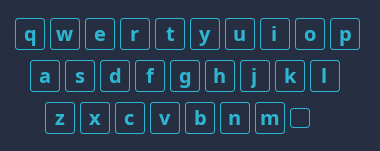
\includegraphics[height=100px,keepaspectratio]{./figures/prethodna_tipkovnica.png}
\end{center}
\smallskip

Također je tražio da ljudi koji koriste aplikaciju imaju uvid u prethodno
odigrane igre u obliku statistika kako bi mogli pratiti:
\begin{itemize}
    \item broj odigranih igara,
    \item broj pobjeda i izgubljenih igara,
    \item duljinu najdulje pogođene riječi, i
    \item najkraći broj pokušaja prije pobjede.
\end{itemize}

\chapter{Analiza zahtjeva}

\section{Izmjena tikovnice}

Na tipkovnicu je potrebno dodati tipku za potvrdu odgovora.

Kako bi se bolje podržale različite rezolucije zaslona, veličina tipka na
na tipkovnici se treba prilagoditi širini zaslona prilikom čega je potrebno
paziti da na velikim zaslonima (npr. tablet, osobno računalo, velika rezolucija)
veličina tipki bude ograničena na neke smislene dimenzije.

S obzirom da veličina zaslona uređaja nije promjenjiva, potrebno je paziti na
slučaj gdje dimenzije komponente koja prikazuje unesene odgovore ne stanu u
prostor između poglavlja aplikacije i tipkovnice te ju omeđiti komponentom koja
dozvoljava vertikalno pomicanje unutarnjeg sadržaja (engl. Scroll Area).

\section{Dodavanje statistike}

Za praćenje statistike igara je potrebno dodati podršku za pohranu odigranih
igara. Dok je tu podršku moguće izvesti korištenjem postojećih mehanizama za
serijalizaciju koji su već prisutni u aplikaciji, zbog performansa dohvata
podataka je bolje rješenje koristiti bazu podataka.

Zbog veličine aplikacije i malog broja primjena, odabir SQLite baze podataka se
doima kao najbolje rješenje.

Odabrana implementacija mora podržavati sve ciljane platforme.

\chapter{Modeliranje grafičkog sučelja}

Aplikacija je velikim djelom već gotova prilikom obrade korisničkih zahtjeva
te je potrebno doraditi model tipkovnice i model zaslona za statistiku.

\section{Tipkovnica}

Popravljen je izgled tipke za brisanje unosa, kao i dodana tipka za potvrdu
unesene riječi:

\smallskip
\begin{center}
    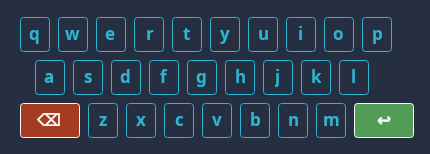
\includegraphics[height=100px,keepaspectratio]{./figures/nova_tipkovnica.png}
\end{center}
\smallskip

Kako sama aplikacija podržava lokalizaciju, i tipkovnica je lokalizirana kroz
lako podesivu JSON datoteku.

\smallskip
\begin{center}
    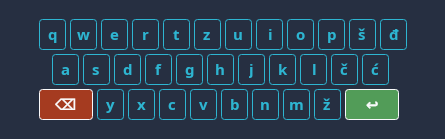
\includegraphics[height=100px,keepaspectratio]{./figures/nova_tipkovnica_hr.png}
\end{center}
\smallskip

Također, prilikom kraja igre se mjenjaju tipke na tipkovnici kako bi bila
jasnija njihova izmjenjena funkcija.

\smallskip
\begin{center}
    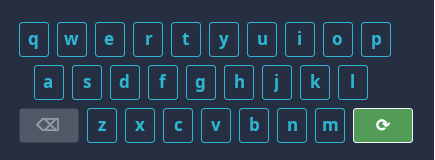
\includegraphics[height=100px,keepaspectratio]{./figures/nova_tipkovnica_1.png}
\end{center}
\smallskip

\newpage
Cijeli početni zaslon sada izgleda ovako:

\smallskip
\begin{center}
    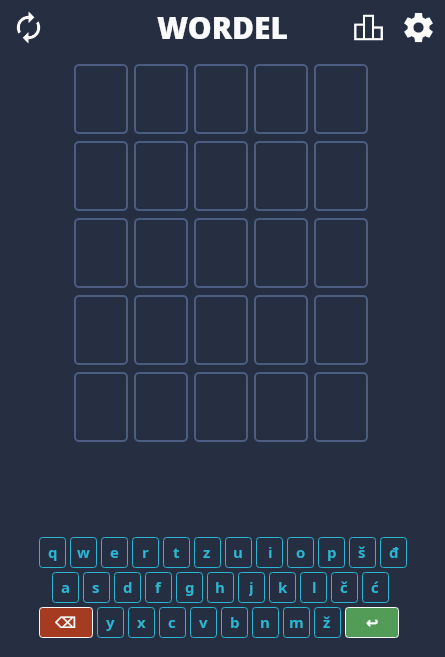
\includegraphics[width=300px,keepaspectratio]{./figures/glavni_zaslon.png}
\end{center}

\newpage
\section{Statistika}

U aplikaciju je dodan sljedeći prikaz za statistike igrača:

\begin{center}
    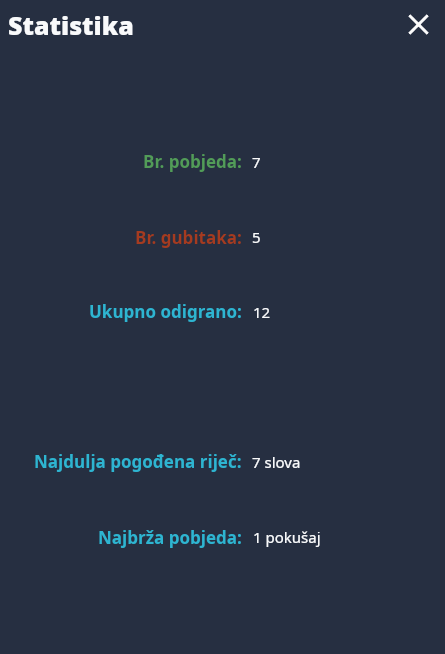
\includegraphics[width=300px,keepaspectratio]{./figures/statistika.png}
\end{center}

Prilikom završavanja igre (pobjeda/gubitak), povratkom na taj zaslon korisnik
može dobiti uvid u svoje odigrane igre.

\chapter{Testiranje}

\section{Testiranje jedinica}
U prethodnim jediničnim testovima se nalazila pogreška zbog čega su davali
netočne rezultate. Ta pogreška je prilikom razvoja bila ispravljena.

Zbog lošeg testa je prilikom inicijalnog razvoja promakla pogreška u izvedbi
algoritma za usporedbu unesene i tražene riječi što potvrđuje bitnost kvalitetne
provedbe testiranja.

Novi skup testova algoritma korištenog u aplikaciji izgleda ovako:

\inputminted{cs}{../Wordel/Wordel.Tests/TextMatchingTest.cs}

\newpage
\section{Testiranje grafičkog sučelja}

Testiranje grafičkog sučelja nije bilo provedeno te je to bio uzrok prvog
naknadnog zahtjeva korisnika.

Nedostatak gumba za unos odgovora ne bi promakao tokom razvoja aplikacije jer bi
pisanje automatiziranog testa koji provjerava osnovne funkcionalnosti ukazao na
taj nedostatak.

Zbog složenosti pisanja automatskih testova, kao i postavljanje okruženja za
njih, te jednostavnosti aplikacije je naknadno bilo odrađeno ručno testiranje na
mobilnom uređaju.

Ručnim testiranjem grafičkog sučelja je osigurano da:
\begin{itemize}
    \item korisnik može pokrenuti igru, unijeti znakove, ukloniti znakove i
          potvrditi unos,
    \item korisnik može otvoriti zaslon sa postavkama te ih izmjeniti,
    \item korisnik može otvoriti zaslon sa statistikama o odigranim igrama te
          se je taj zaslon ažuran prilikom otvaranja, te da su
    \item tipke na tipkovnici prikladnih dimenzija neovisno o veličini
          zaslona ili prozora.
\end{itemize}

Sa zaključkom ovog seminarskog rada, Android inačica aplikacije je u potpunosti
testirana i funkcionalna na mobilnim uređajima.

\section{Testiranje od strane korisnika}

Pri završetku razvoja, bilo je provedeno i testiranje među korisnicima koji
spadaju u ciljane grupe.

Prilikom ovog testiranja su korisnici izrazili potrebu za dodatnim povečanjem
visine tipkovnice te je to bilo naknadno provedeno.

\chapter{Razvoj aplikacije}

Za razvoj aplikacije je bila korištena Avalonia UI platforma koja podržava
mobilne platforme. Za kod je bio korišten C\# programski jezik koji kroz
\verb|Xamarin| platformu podržava kompajliranje na Android platformu.

To je izvedeno tako što je \verb|Mono| radno okruženje (engl. runtime) upakirano
u proizvedenu aplikaciju (apk), zajedno s kodom koji komunicira sa Javom kroz
\verb|JNI| (Java native interface) sučelje.

Rezultat toga je da su aplikacije složene na ovaj način nešto veče od
Java/Kotlin aplikacija, no sjedinjuje se razvoj prilikom ciljane podrške više
različitih platforma.

\section{SQLite}

Za korištenje SQLite baze podataka je bila upotrijebljena \verb|sqlite-net-pcl|
biblioteka te upakirana \verb|SQLitePCLRaw| implementacija.
\verb|sqlite-net-pcl| biblioteka je radila na desktop verziji bez dodatnih
zavisnosti, no na Androidu je bilo potrebno dodati \verb|SQLitePCLRaw| zbog
nedostajučih dinamičkih biblioteka\\(\verb|SQLitePCLRaw.provider.sqlite3.so|).

Korištenje same biblioteke je bilo iznimno jednostavno. Uključen je jednostavan
ORM koji pomoću refleksije generira SQL zahtjeve za stvaranje tablica, pohranu
podataka, te čitanje spremljenih podataka. Po tome je \verb|sqlite-net-pcl|
dosta slična \verb|Room| biblioteci koja je dio \textit{Android Jetpack}a.

\verb|sqlite-net-pcl| biblioteka je jednostavnija za koristiti, no nedostaju joj
mnoge značajke koje \verb|Room| ima - poput definiranja automatskih migracija.

Dodana baza se sastoji od jedne tablice koja pohranjuje odigrane igre:

\inputminted{cs}{../Wordel/Wordel/Data/PlayedGame.cs}
\newpage

Za manipulaciju baze podataka je bila složena \verb|Database| singleton klasa
koja prilikom stvaranja otvara/stvara datoteku za pohranu sukladno platformi
na kojoj je aplikacija pokrenuta:

\inputminted[breaklines]{cs}{../Wordel/Wordel/Data/Database.cs}

\verb|GetStats| funcija se koristi za prikupljanje podataka prikazanih u zaslonu
sa statistikama. \verb|sqlite-net-pcl| dozvoljava pisanje nekih jednostavnijih
zahtjeva direktno u C\#u (poput \verb|quickest|), no za neke složenije zahtjeve
je potreno koristiti \verb|Query| funkciju.

\newpage
\section{Tipkovnica}

Za tipkovnicu je korišten sljedeći kod koji ju generira ovisno o trenutno
odabranom jeziku sučelja\footnote[1]{posebni znakovi \verb|Content| članova su
zamjenjeni svojim značajem zbog neispravnog prikaza}, naspram originalne verzije
je dodan kod koji računa širine i visine gumba za unos:

\begin{minted}[breaklines]{cs}
private void RebuildKeyboard()
{
    if (DataContext is not GameViewModel model) return;
    
    KeyboardStackPanel.Children.Clear();
    var rowWidth = ((Grid?) KeyboardStackPanel.Parent)?.Bounds.Width ?? 440.0;
    
    var rows = LocaleStorage.CurrentLocale!.Keyboard.lower;
    var keySpacing = 8.0;
    var keyWidth = rowWidth / rows[0].Length - (6.0 + keySpacing);
    switch (keyWidth)
    {
        case > 50.0:
            keySpacing = 9.0;
            keyWidth = 50.0;
            break;
        case < 26.0:
            keySpacing -= 4.0;
            keyWidth += 4.0;
            break;
    }
    var keyHeight = keyWidth * 1.15;
    var fontSize = keyHeight * 0.5;

    KeyboardStackPanel.Spacing = keySpacing;
    
    foreach (var row in rows)
    {
        var currentRow = new StackPanel();
        currentRow.Orientation = Orientation.Horizontal;
        currentRow.Spacing = keySpacing;

        if (KeyboardStackPanel.Children.Count != 2)
        {
            currentRow.Margin = new Thickness((keyWidth / 2.0) * KeyboardStackPanel.Children.Count, 0, 0, 0);
        }
        else
        {
            currentRow.Margin = new Thickness((keyWidth / 2.0) * KeyboardStackPanel.Children.Count - keyWidth, 0, 0, 0);
        }
        
        if (KeyboardStackPanel.Children.Count == 2)
        {
            var eraseButton = new Button
            {
                Content = "erase",
                Command = ReactiveCommand.Create(model.RemoveLetter),
                Padding = new Thickness(),
                Width = keyWidth * 2.0,
                Height = keyHeight,
                    FontSize = fontSize,
                IsEnabled = model.Status == GameStatus.Play
            };
            eraseButton.Classes.Add("keyboard");
            eraseButton.Classes.Add("erase");
            currentRow.Children.Add(eraseButton);
        }
        
        foreach (var letter in row)
        {
            var button = new Button
            {
                Content = letter.ToString(),
                Command = ReactiveCommand.Create(() =>
                {
                    model.EnterLetter(letter);
                }),
                Padding = new Thickness(),
                Width = keyWidth,
                Height = keyHeight,
                FontSize = fontSize,
            };
            button.Classes.Add("keyboard");
            currentRow.Children.Add(button);
        }
        
        if (KeyboardStackPanel.Children.Count == 2)
        {
            var confirmButton = new Button
            {
                Content = model.Status == GameStatus.Play ? "confirm" : "reset",
                Command = ReactiveCommand.Create(model.ConfirmAnswer),
                Padding = new Thickness(),
                Width = keyWidth * 2.0,
                Height = keyHeight,
                FontSize = fontSize,
            };
            confirmButton.Classes.Add("keyboard");
            confirmButton.Classes.Add("confirm");
            currentRow.Children.Add(confirmButton);
        }

        KeyboardStackPanel.Children.Add(currentRow);
    }
}    
\end{minted}

\verb|LocaleStorage.CurrentLocale!.Keyboard| je \verb|HashMap|a koja sadrži
znakove tipaka, i učitava se iz JSON datoteke sljedećeg oblika:

\inputminted{json}{../Assets/i18n/keyboard.hr.json}

Time je osigurana iznimno jednostavna podrška unosa zvih potrebnih znakova
neovisno o korištenom jeziku.

\newpage
\section{Korisničko sučelje}

Korisničko sučelje je složeno pomoću \verb|AUI|, strukturirano \verb|MVVM|
arhitekturom.

\subsection{MVVM arhitektura}

Za korisnička sučelja je bila korištena MVVM arhitektura koja rasčlanjuje
detalje implementacije sučelja na:

\textbf{Model} - sloj aplikacije zaslužan za definiranje podatkovnih struktura
aplikacije.

\textbf{Pogled (engl. View)} - sloj aplikacije zaslužan za slaganje i prikaz
komponenti s kojima korisnik interagira.

\textbf{Model pogleda (engl. View Model)} - sloj aplikacije namijenjen pohrani i
manipulaciji modela, kao i definiranju izvora događaja za reaktivnost.

Za razliku od Android Studia, za Avalonia UI ne postoji WYSIWYG editor
komponenta i prikaza, no oni su također deklarirani u jednostavnim XML
datotekama tako da nije bilo večih komplikacija prilikom izrade sučelja.

\subsubsection{Pogledi}

Prikaz statistika ima sljedeći oblik u \verb|.axaml| datoteci:

\inputminted[breaklines,breakanywhere,fontsize=\scriptsize]{xml}{../Wordel/Wordel/Views/StatsView.axaml}

Uz tu datoteku je potrebno definirati i istoimenu \verb|.axaml.cs| datoteku u
kojoj su implementirane funkcije koje definiraju ponašanje prilikom događaja:

\inputminted[breaklines]{cs}{../Wordel/Wordel/Views/StatsView.axaml.cs}

Takav pristup odjeljuje detalje izvedbe od strukture sučelja čime se dozvoljava
razvoj specijaliziranih alata za uređivanje grafičkih sučelja poput
\href{https://gluonhq.com/}{Gluon}a, ali i odjeljuje dizajn od razvoja softvera
čime se omogućuje dizejniranje sučelja i ljudima koji nisu upoznati sa
programiranjem ili korištenim programskim jezikom.

\subsubsection{Modeli pogleda}

Model pogleda za statistike sadrži funkcije koje dohvaćaju lokalizirani
prikazani tekst, kao i podatke koji su prikazani na ekranu. Za slučaj prikaz
statistika takav model pogleda ima sljedeći oblik:

\inputminted[breaklines]{cs}{../Wordel/Wordel/ViewModels/StatsViewModel.cs}

\subsubsection{Modeli}

Prilikom rada sa podacima koji su spremljeni u bazi podataka, funkcije baze
podataka vraćaju strukturirane podatke. Kako bi se odvojilo grafičko sučelje od
ostatka koda su oni definirani u \verb|PlayStats.cs| datoteci:

\inputminted{cs}{../Wordel/Wordel/Model/PlayStats.cs}

Tako je osigurano da:
\begin{itemize}
    \item pogled ne treba znati detalje o implementaciji i ostatku koda te je
          zbog toga lagan za izmjeniti,
    \item model je zaokružena cjelina koja ne ovisi o ostalim djelovima koda
          što ga čini manje podložnom pogreškama, te da
    \item se model može koristiti u cijeloj aplikaciji bez da ostatak koda bude
          vezan za detalje o grafičkom sučelju.
\end{itemize}

\newpage
\subsection{Izrada komponenta}

Često je prilikom razvoja korisničkih sučelja poželjno ponoviti neke komponente
na nekoliko različitih mjesta. Zbog DRY (don't repeat yourself; ne ponavljaj se)
principa, večina platforma za izradu grafičkih sučelja dozvoljava programerima
da definiraju svoje komoponente. Često je to i poželjno napraviti kako bi
dobiveni kod bio pregledniji.

Također, često želimo stvoriti komponente koje su jedinstvene za našu aplikaciju
ili imaju dovoljno jedinstven izgled ili interakciju, da ih nije moguće
ostvariti korištenjem (stiliziranih) postojećih komponenta. U tom slučaju večina
platforma za izradu grafičkih sučelja dozvoljava komponentama da specificiraju
vlastitu logiku za čitanje događaja (npr. klik na miš) i logiku za crtanje
komponenta.

Wordel definira dvije takve komponente, koje se u kontekstu Avalonie zovu
\verb|TemplatedControl|:

\textbf{IconButton} je primjer prve primjene gdje je zbog učestalog
pojavljivanja gumba koji sadrže samo ikonu (bez teksta) bila složena jednostavna
komponenta za tu namjenu.

\textbf{AnswerField} je primjer druge primjene gdje je bio poželjan stiliziranih
prikaz unesenih odgovora te je to ostvareno sa preopterećivanjem \verb|Render|
funkcije na komponenti.

U Avalonia platformi se crtanje provodi kroz \verb|DrawingContext| instancu
prosljeđenu \verb|Render| funkciji koja interno stvara pozive bibliotekama za
crtanje zavisno o platformi na kojoj se aplikacija pokreće. Generalno se radi o
\verb|OpenGL|u, no novije platforme često imaju podršku i za \verb|Vulkan|.
U slučaju Androida se pretežno koristi \verb|OpenGL ES| koji je pojednostavljena
verzija \verb|OpenGL|a za jednostavnije grafičke uređaje.

Android SDK također sadrži takvu funkciju koja se može preopteretiti pod nazivom
\verb|onDraw|. Ona prima \verb|Context| (kontekst za crtanje) koji za razliku od
Avaloniinog \verb|DrawingContext|a sadrži interno stanje te se nacrtani sadržaj
tako podešava.

\section{Učitavanje resursa}

Avalonia UI uključuje dio koda koji podržava učitavanje resursa koji su
upakirani u binarni kod aplikacije. Kako bi ih kompajler upakirao u binarni kod,
potrebno ih je smjestiti u predodređenu \verb|Assets| datoteku, ili naznačiti u
\verb|.csproj| datoteci da je tip datoteke sa danom putanjom
\verb|AvaloniaResource|.

Komponente poput \verb|Icon| su osposobljene same učitati resurse sa putanje
koja im je predana kroz \verb|Source| parametar. No ako je resurs potreban u
drugom dijelu koda, moguće mu je pristupiti kroz statične funkciju \verb|Open|
na \verb|AssetLoader| klasi.

Kroz \verb|AssetLoader| je osiguran mehanizam gdje aplikacija prvo pokušava
učitati resurse sa korisnikovog datotečnog sustava, te u slučaju da ih nema ih
se pokuša raspakirati iz aplikacije, te ako se ne nalaze niti u aplikaciji,
dohvatiti sa git-a. To dozvoljava korisnicima da dodaju svoj jezik ili riječi
u riječnik bez potrebe za pristupom izvornom kodu aplikacije ili za
kompajliranjem nove binarne datoteke.

\section{Postavke}

Za zaslon sa postavkama se zbog jednostavnosti kasnijeg proširivanja postavki
koristila refleksija.

Bio je definiran \verb|Configurable| atribut koji kroz primjenu na članove klase
\\\verb|Settings| dozvoljava automatsko generiranje polja za upravljanje
njihovim vrijednostima.

Ovaj pristup dozvoljava iznimno laganu i brzu iteraciju nad prikazanim sadržajem
po cijenu performansa prilikom izvođenja aplikacije. U \verb|DEBUG| varijanti
aplikacije se osjeti zastoj od $\text{~}500\text{ms}$ prilikom paljenja tog
zaslona, no bolja izvedba bi to mogla izbjeći za pokretanjem takvog koda prije
nego je rezultat potreban (krajem pokretanja aplikacije).

Nedostatak takvog pristupa je to što je potrebno unaprijed napisati kod koji
upravlja ponašanjem aplikacije na osnovu pronađenih podataka:

\begin{minted}[breaklines]{cs}
private void BuildOptions()
{
    var model = (DataContext as SettingsViewModel)!;
    OptionsGrid.Children.Clear();
    OptionsGrid.ColumnDefinitions = new ColumnDefinitions("*,Auto");
    
    var rowDefs = new RowDefinitions();
    var row = 0;

    var fields = model.SettingFields;
    foreach (var (field, conf) in fields)
    {
        var label = new TextPresenter
        {
            Margin = new Thickness(10, 0, 0, 0),
            VerticalAlignment = VerticalAlignment.Center,
            TextAlignment = TextAlignment.Left,
            FontSize = 18,
            Text = LocaleStorage.GetTranslation(field.Name + "SettingsOption")
        };
        label.SetValue(Grid.ColumnProperty, 0);
        label.SetValue(Grid.RowProperty, row);
        OptionsGrid.Children.Add(label);

        Control? control = null;
        switch (conf.Kind)
        {
            case ConfigKind.Integer:
            {
                var value = new NumericUpDown
                {
                    Margin = new Thickness(0, 0, 10, 0),
                    Width = 150,
                    Increment = conf.Increment ?? new decimal(1.0),
                    HorizontalContentAlignment = HorizontalAlignment.Right,
                    Value = new decimal((int?) field.GetValue(model.Settings) ?? (int?) conf.Default ?? 0.0)
                };
                if (conf.Limits.HasValue)
                {
                    value.Minimum = new decimal((int) conf.Limits.Value.Item1);
                    value.Maximum = new decimal((int) conf.Limits.Value.Item2);
                }
                value.AddHandler(NumericUpDown.ValueChangedEvent, (sender, args) =>
                {
                    if (!args.NewValue.HasValue) return;
                    field.SetValue(model.Settings, (int) args.NewValue);
                });
                
                control = value;
                break;
            }
            /* Kod za ostale vrste postavki */
        }
        if (control == null) continue;
        
        control.SetValue(Grid.ColumnProperty, 1);
        control.SetValue(Grid.RowProperty, row);
        OptionsGrid.Children.Add(control);
        rowDefs.Add(new RowDefinition(GridLength.Auto));
        row += 1;
    }
    
    OptionsGrid.RowDefinitions = rowDefs;
}
\end{minted}

\newpage
No nakon što smo naveli logiku koja podržava sve željene ciljeve, daljnji razvoj
koda postaje iznimno učinkovit i dobivamo vrlo pregledan kod. Tako se model
\verb|Settings| sastoji od samo 20 linija koda i \verb|SettingsView| ne zahtjeva
naknadnu doradu prilikom dodavanja postavka:

\inputminted{cs}{../Wordel/Wordel/Model/Settings.cs}

Refleksija je koristan alat za introspekciju u kodu koji je dostupan u večini
dinamičnih jezika.

\chapter{Daljni razvoj}

Wordel projekt je moguće dalje poboljšati:
\begin{itemize}
    \item spremanjem stanja igre u toku te povratak na njega prilikom izmjene
          aktivnog pregleda,
    \item dodavanjem podrške za podešavanje visine tipkovnice,
    \item pametnijim odabirom tražene riječi u novim igrama,
    \item dodavanjem mogučnosti ručnog unosa tražene riječi ili drugog oblika
          djeljenja trenutne igre s drugim korisnicima,
    \item dodavanjem zvukova za interakcije (tipkovnica),
    \item dodavanjem animacija, te
    \item dodavanjem podrške za više jezika.
\end{itemize}

\end{document}
